\chapter{A Color X-ray Camera for 2 -- 6 keV Using a Mass-Produced CMOS Sensor}
\label{cmos_ch2}
Oliver R. Hoidn\textsuperscript{1}, William M.
Holden\textsuperscript{1}, and Gerald T. Seidler\textsuperscript{1,*}

\textsuperscript{1}Physics Department, University of Washington, Seattle
WA 98195-1560

(*) \href{mailto:Seidler@uw.edu}{seidler@uw.edu}

\section{Abstract}
We report here the development of an x-ray camera for 2 -- 6 keV photons
using mass-produced sensors and commercial control electronics. This
instrument has several favorable characteristics for advanced x-ray
spectroscopy studies in the laboratory, at synchrotron light sources, at
x-ray free electron lasers, or using pulsed x-ray sources such as for
laser plasma physics research. These characteristics include fine
position and energy resolution for individual photon events; high
saturation rates; easy user maintenance for damaged sensors; and
software for real-time processing. We present results that evaluate this
camera for use a as an alternative to traditional energy-dispersive
solid-state detectors, such as silicon drift detectors, and also
illustrate its use in a dispersive x-ray emission spectrometer that has
recently been reported elsewhere (Holden, et al., 2017).

\section{Introduction}
The capabilities of a variety of x-ray techniques at the synchrotron,
x-ray free electron laser (XFEL) and university-scale laboratory are
heavily dependent on the characteristics of the x-ray detectors with
which they are implemented. One technological regime of interest is that
of pixel area detectors combining spectroscopic and spatial resolution
with features such as high readout rate, large collection solid angle,
and hardness to ionizing radiation and electromagnetic pulses (EMPs).
The advent of time-resolved spectroscopy with pulsed photon sources,
such as x-ray free electron lasers (XFELs), where it is often necessary
to collect large numbers of signal photons quasi-instantaneously and
with repetition rates exceeding 100 Hz, has greatly expanded the need
for this class of detectors. Similar needs are also present in
laser-plasma physics, where entire spectra for fluorescence, x-ray band
thermal emission, or inelastic scattering must often be collected in
truly single-pulse experiments.

While there is an impressive effort aimed at either improvement of
existing state-of-the-art technology or \emph{de novo} development of
new ideas for truly advanced high-performance detectors, there is
another route that requires consideration. Highly mass-produced,
commercial multipixel sensors intended for primary use at optical
wavelengths are, by the standards of x-ray science, already stunningly
advanced sensors. For example, recent advances in the performance of
mass-produced CMOS image sensors, including readout rates above 200
Mpix/second and optical-wavelength quantum efficiencies exceeding 80\%,
significantly increases their potential for scientific applications. The
direct application of such sensors to the x-ray regime is limited mainly
by the fact that their small pixel thicknesses lead to greatly decreased
quantum efficiency for hard x-rays. That being said, the use of CMOS
image sensors in the x-ray regime has been explored in prior literature,
which has established them as viable spectroscopic imaging detectors
having a favorable combination of low cost (a consequence of chip-level
integration of all sensor functions), high framerates, and improved
radiation hardness relative to comparable charge coupled devices (CCDs).
\textsuperscript{1-4}. By `spectroscopic', we mean that the camera
output contains sufficient information for determination of both the
energy and position of a photoabsorbed x-ray-- such devices are often
referred to as `color x-ray cameras'.

In a prior publication we presented an x-ray camera platform for the 2-6
keV photon energy range based on a legacy CMOS image sensor, the Aptina
MT9M001. Here, we introduce a new camera that incorporates a modern
back-illuminated CMOS sensor with significantly improved readout rates
and finer spectral and positional resolution compared to the previous
model. We find an energy resolution of \textasciitilde{}150 eV at 2 keV
with saturation rates above 10\textsuperscript{6}/s at
\textasciitilde{}80 Hz frame rate. These spectroscopic benefits are
complemented by a spatial resolution of 2.9 µm and real-time processing
of all results, but are constrained by a \textasciitilde{}65\% quantum
efficiency at 2 keV that decreases to below 20\% at 5 keV.

This manuscript continues as follows. First, in section II, we describe
the commercial hardware, and its modification used in the present
instruments, and also the new software package that has been developed
to support real-time spectral analysis or real-time energy-windowed
imaging. A key point here is that it is not only the sensor, but also
the entire camera read-out system that is commercially available because
of the high demand for extreme low-light sensitivity for, e.g., amateur
astronomy. Next, in section III, we present results and discussion,
demonstrating the cluster-binning methods and also both
energy-dispersive and photon-counting modes for the camera. This
includes representative data from a wavelength-dispersive spectrometer
whose design has recently been described elsewhere. \textsuperscript{5}
Finally, in section IV we conclude and provide future directions.

\section{II. Experimental }

\subsection{II.A. Hardware}

The hardware consists of a commercial amateur astronomy camera (ZWO
Company) based on the Sony IMX290, a back-illuminated CMOS image sensor
with a rolling shutter, pixel pitch of 2.9-µm, pixel grid of 1936×1096,
and maximum framerate of 170 fps. The sensor features high sensitivity
and dynamic range, with a 12-bit A/D converter and readout noise of 1e-
at maximum analog gain. The choice of vendor and model was driven by the
manufacturer's provision of a software API allowing straightforward
configuration and access to the sensor's uncompressed video stream;
notably, however, other manufacturers offer products with similar
feature sets.

We have modified the camera in two ways. First, the main camera board
has been reworked by removing the IMX290 sensor and replacing it with a
custom IC socket (Andon Electronics). This was done to more easily allow
sensor replacement if radiation damage occurred. Second, the sensor
itself has been modified by removal of the glass cover (Pacific X-Ray).
A photo of the resulting camera is shown in Fig. \ref{cmos2_image1}. The yellow plastic
part holding down the sensor is a simple clamp used to press the sensor
against the socket contact pads.

\begin{figure}[h] \label{cmos2_image1}
\caption{ Photograph of the modified camera. The original commercial
product has been reworked to install an IC socket for the sensor and to
remove the glass cover of the sensor.}
\centering
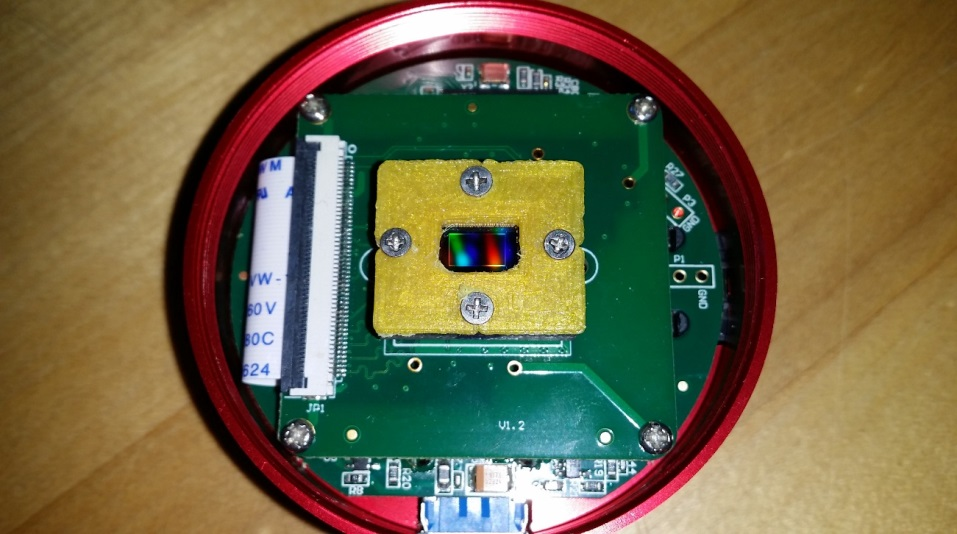
\includegraphics{cmos2/image1.jpeg}
\end{figure}

\subsection{II.B. Software}

Charge separation generated by an x-ray photon absorbed in the active
layer of a sensor pixel results in a signal with expectation value
proportional to the photon's energy. In the simplest case, wherein the
entire charge cloud from an x-ray absorption event is concentrated in a
single pixel, the detecting pixel has intrinsic sensitivity to the
energy of the incident x-ray photon. In the majority of events, however,
the charge cloud spreads over a cluster of several adjacent
pixels.\textsuperscript{3, 4} We have found that, in order to optimize
the camera's quantum efficiency (QE) and spectroscopic sensitivity, it
is essential to use this prior information to recover the energy and
position of each detected photon on an event-by-event basis. To do this
we perform a ``breadth-first'' search\textsuperscript{6} of every frame
to identify sets of connected pixels with ADC values above a
user-specified signal threshold For each cluster thus identified, the
signal is summed over all member pixels and the event's position is
inferred from the cluster's center of mass. This technique is similar to
event-reconstruction algorithms used for the same purpose in prior
literature, with the difference that we place no constraint on the size
and shape of signal clusters \textsuperscript{3}\emph{.} The sensor's
low noise floor (under 1 e- per pixel) (\emph{cite datasheet. Can't find
anything about the citation format for datasheets under the AIP style
guide)} allows the use of an aggressively low threshold level, resulting
in a high level of signal.

To implement the above analysis while avoiding the prohibitively large
quantity of disk storage that offline processing demands, we developed a
real-time data processing pipeline; the general framework for this
pipeline is shown in Fig. \ref{cmos2_image2}. It consists of a collection of several
software components communicating with one another over ZeroMQ sockets.
First, a customized version of the open source image capture program
oaCapture controls the camera's readout, allowing the user to configure
the camera's gain and per-frame exposure time. Event reconstruction,
which requires the computational throughput of multiple CPU cores, is
done by a pool of worker processes collecting frames from the capture
application in round-robin fashion. The resulting filtered frames from
this parallel pipeline are aggregated on a sink node that communicates
with an API component that, in turn, provides users with high-level
functions for acquiring and visualizing pre-processed camera data.

\begin{figure}[h] \label{cmos2_image2}
\caption{ Diagram of camera data processing pipeline.
}
\centering
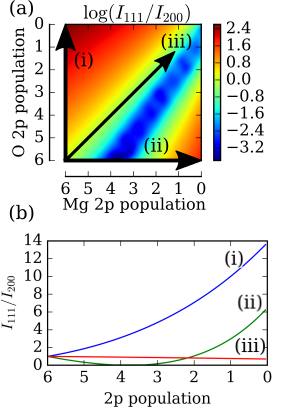
\includegraphics[scale=0.40]{cmos2/image2.png}
\end{figure}

\section{III. Results and Discussion}

In this section we address four aspects of the camera operation and
performance: the cluster algorithm, energy dispersive operation, quantum
efficiency, and finally single-photon counting mode for
spectroscopically-constrained imaging. First, a magnified view of a
small region of a captured image is presented in Fig. \ref{cmos2_image4}, where
single-photon signal clusters are readily identifiable. The distribution
of cluster sizes is strongly skewed; the largest clusters contain more
than 10 pixels, while the mean number is 2.1.

\begin{figure}[h] \label{cmos2_image4}
\caption{
 Representative cropped region of a camera frame during direct
illumination by a Rh anode x-ray tube source operating at 6 kV bias
voltage, with the camera detecting 2 $\times$ 10\textsuperscript{6} photons/s
at an 80 Hz frame rate.
}
\centering
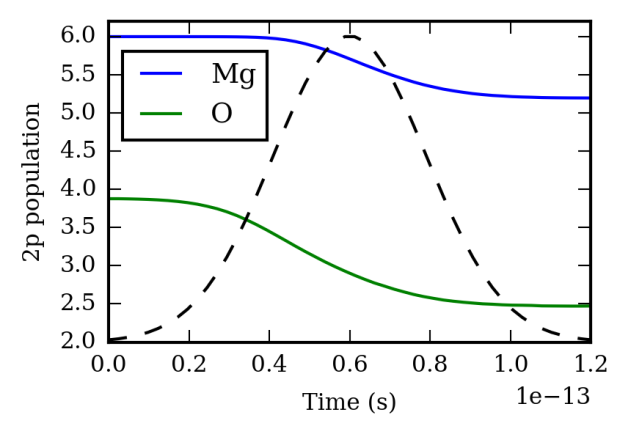
\includegraphics{cmos2/image4.png}
\end{figure}

Second, when operated as a spectroscopic sensor, the camera's
user-visible output is a histogram, summed over all frames, of number of
events binned by per-event signal. This is demonstrated in Fig. \ref{cmos2_image6} (top
panel), which shows the direct-illumination spectrum of a laboratory
x-ray tube source. The dominant components of the signal are the tube's
continuous bremsstrahlung spectrum and Rh L-shell emission from the
anode. Two detector artifacts are also visible. First, a peak at the
energy of Si Kα is generated by Si fluorescence photons emitted in the
sensor that propagate far enough from their originating interaction
sites to be registered as separate events. Second, the escape of Si
fluorescence from the absorption sites of Rh L photons creates echos of
the Rh L peaks (termed escape peaks) that are downshifted by 1.74 keV,
the energy of Si Kα. We find that the camera's energy resolution at the
energy of P Kα is 150 eV (Fig. \ref{cmos2_image6} bottom panel), somewhat inferior to
SDD's at this energy but still sufficient for many applications.

\begin{figure}[h] \label{cmos2_image6}
\caption{
 Energy dispersive spectrum from direct illumination of the
camera by a Rh anode x-ray tube source operating at 6 keV bias voltage.
The ADC channel at the peak of the Rh L emission contains \(^{}\)
counts. See the text for discussion.
}
\centering
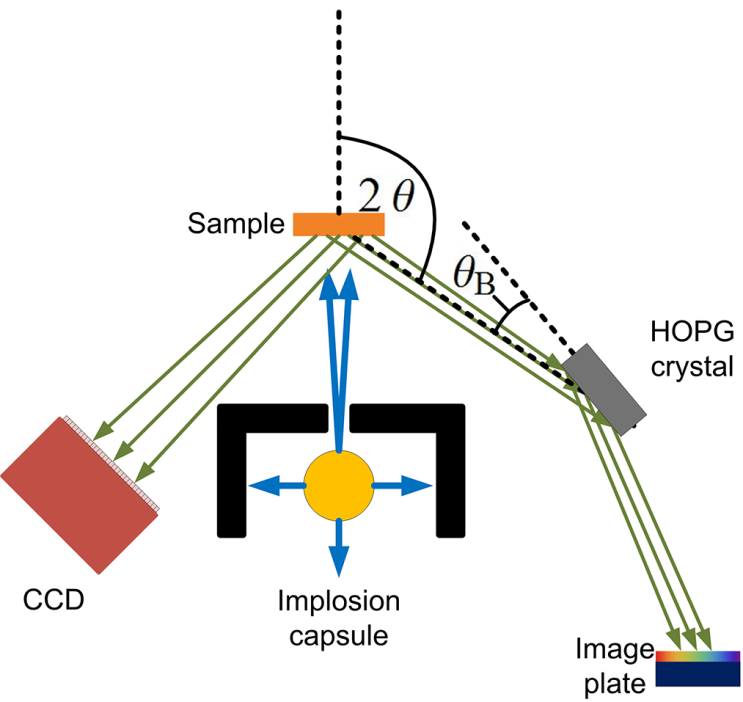
\includegraphics{cmos2/image6.png}
\end{figure}

Third, the quantum efficiency (QE) of the detector was characterized by
measurement of the K-shell fluorescence spectra of several elements,
using a low-power laboratory x-ray tube source to excite 1s core holes
in each measured sample. The intensity of resulting Kα and Kβ emission
registered by the detector was referenced to that recorded at the same
position by a commercial Si drift detector (Amptek XR-100SDD) having
known QE. Results are presented in Fig. \ref{cmos2_image7}; we note a maximum QE of 60\%
at the energy of P Kα, a more than two-fold improvement over our
previous camera.\textsuperscript{4} Under uniform illumination from Rh
x-ray tube at 6 kV accelerating potential, the observed count rates
have only minimal deviations from linearity at count rates up to 2 x
10\textsuperscript{6} photons per second 80 Hz frame rate (see Fig. \ref{cmos2_image9})
-- an impressive performance that is higher than the typical saturation
rate of commercial silicon drift detectors. The lower count rates for
the CMOS camera compared to the SDD are a consequence of the camera's
lower quantum efficiency at higher photon energies.

\begin{figure}[h] 
\caption{
 Camera count rate as a function of incident photon intensity,
controlled via current provided to an x ray tube source directly
illuminating the camera (blue). We compare to the same curves for a
commercial SDD with pulse shaping times optimized for count rate
(orange) and energy resolution (green). The camera's saturation count
rate is a factor of approximately 10 higher than the SDD's. The low
efficiency of the camera is due to the high flux at higher photon
energies, see Figures \ref{cmos2_image7} and \ref{cmos2_image9}.
}\label{cmos2_image9}
\centering
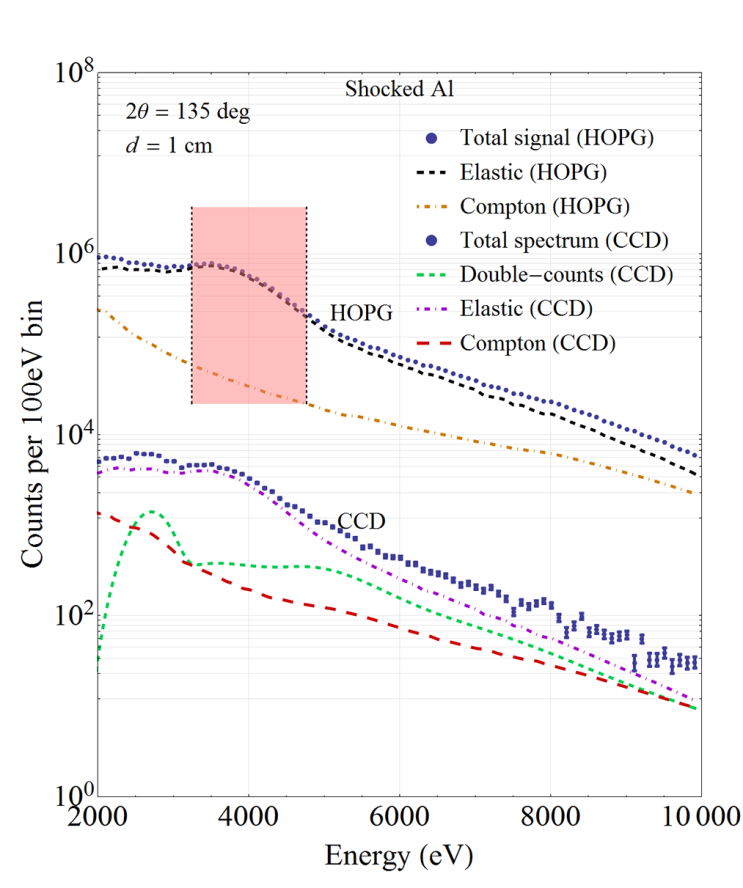
\includegraphics{cmos2/image9.png}
\end{figure}

\begin{figure}[h] \label{cmos2_image7}
\caption{
 The camera's quantum efficiency as a function of x-ray photon
energy, as established by comparison with a commercial Si drift
detector.
}
\centering
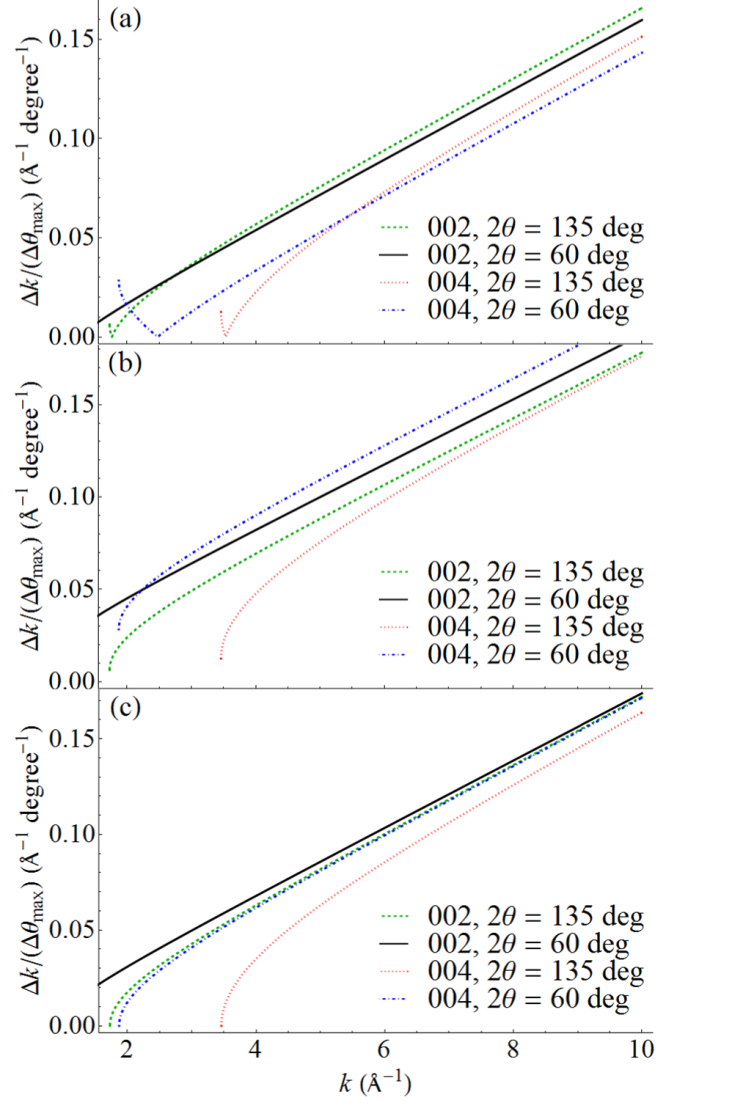
\includegraphics{cmos2/image7.png}
\end{figure}

Finally, the camera's combination of high saturation count rates and
small pixel dimension makes it a strong fit as a position-sensitive
detector in compact dispersive x-ray emission spectrometer designs. In
such an application the camera's spectroscopic sensitivity may be
employed for background rejection (i.e., for rejection of photons with
energies outside a pre-specified range), thus minimizing the need for
shielding from stray scatter. Holden et al. have demonstrated this
advantage in a novel compact dispersive refocusing Rowland (DRR)
spectrometer design with a 10 cm-Rowland circle that incorporates the
camera as its position-sensitive detector (Fig. \ref{cmos2_image11}). The spectrometer's
small dimensions, which are enabled in part by the camera's fine spatial
resolution, give it a large collection efficiency which results in count
rates in laboratory studies (using low-power x-ray tube sources)
comparable to those at a third-generation synchrotron insertion device.
The instrument has thus far been demonstrated in the university-scale
laboratory and at the synchrotron; its potential use at the Linac
Coherent Light Source (LCLS) is currently being investigated, especially
as the sensor frame rate can likely be matched to the 120 Hz repetition
rate of that XFEL.

\begin{figure}[h] \label{cmos2_image11}
\caption{
 Image of the sensor's output when serving as the
position-sensitive area detector in a DRR spectrometer.
\textsuperscript{5} The signal shown is a S k alpha spectrum. In order
to reduce the background level, the camera was configured to reject all
events with photon energies outside of the spectrometer's bandwidth
}
\centering
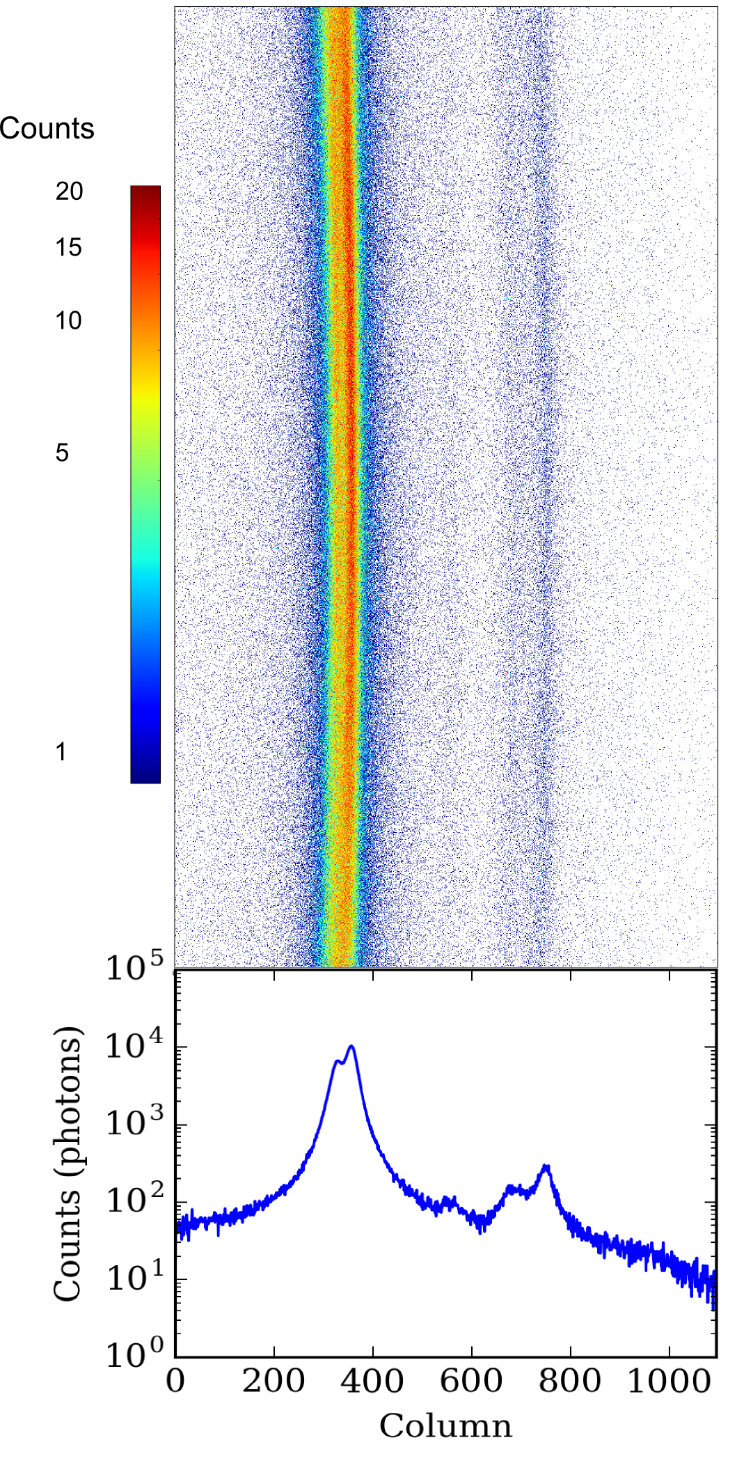
\includegraphics{cmos2/image11.png}
\end{figure}

\FloatBarrier

\section{IV. Conclusions and Future Directions}

In conclusion, we have reported the development of a quite capable x-ray
camera based on a mass-produced consumer product. The observed
performance suggests a range of potential applications as a high-speed
spectroscopic detector with fine spatial resolution and adequate quantum
efficiency in the 2 - 6 keV photon energy range. Among these
applications, we have demonstrated effective use of the camera as a
position-sensitive detector in a novel high-performance compact
dispersive spectrometer.


\section{References}
% TODO: citations

\emph{\\}









